% XCircuit output "pn_kapacita.tex" for LaTeX input from pn_kapacita.ps
\def\putbox#1#2#3#4{\makebox[0in][l]{\makebox[#1][l]{}\raisebox{\baselineskip}[0in][0in]{\raisebox{#2}[0in][0in]{\scalebox{#3}{#4}}}}}
\def\rightbox#1{\makebox[0in][r]{#1}}
\def\centbox#1{\makebox[0in]{#1}}
\def\topbox#1{\raisebox{-0.60\baselineskip}[0in][0in]{#1}}
\def\midbox#1{\raisebox{-0.20\baselineskip}[0in][0in]{#1}}
   \scalebox{0.8}{
   \normalsize
   \parbox{2.72917in}{
   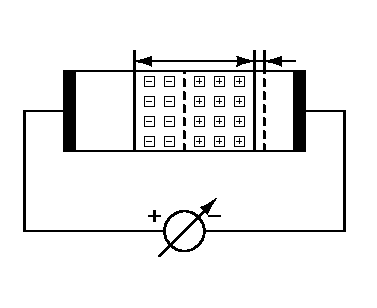
\includegraphics[scale=1.25]{pn_kapacita}\\
   % translate x=719 y=451 scale 0.30
   \putbox{1.90in}{2.09in}{1.20}{$\dif{W}$}%
   \putbox{1.31in}{2.09in}{1.20}{$W_D$}%
   \putbox{1.15in}{0.09in}{1.20}{$U_{0}+\dif{U}$}%
   } % close 'parbox'
   } % close 'scalebox'
   \vspace{-\baselineskip} % this is not necessary, but looks better
